\documentclass[tikz,border=8pt]{standalone}
\usepackage{amsmath}
\usetikzlibrary{arrows.meta,calc,decorations.pathmorphing}
\definecolor{ink}{HTML}{21352F}
\definecolor{teal}{HTML}{087F7B}
\definecolor{blue}{HTML}{4B77A8}
\definecolor{gold}{HTML}{C58B2A}
\definecolor{rose}{HTML}{B65A62}
\begin{document}
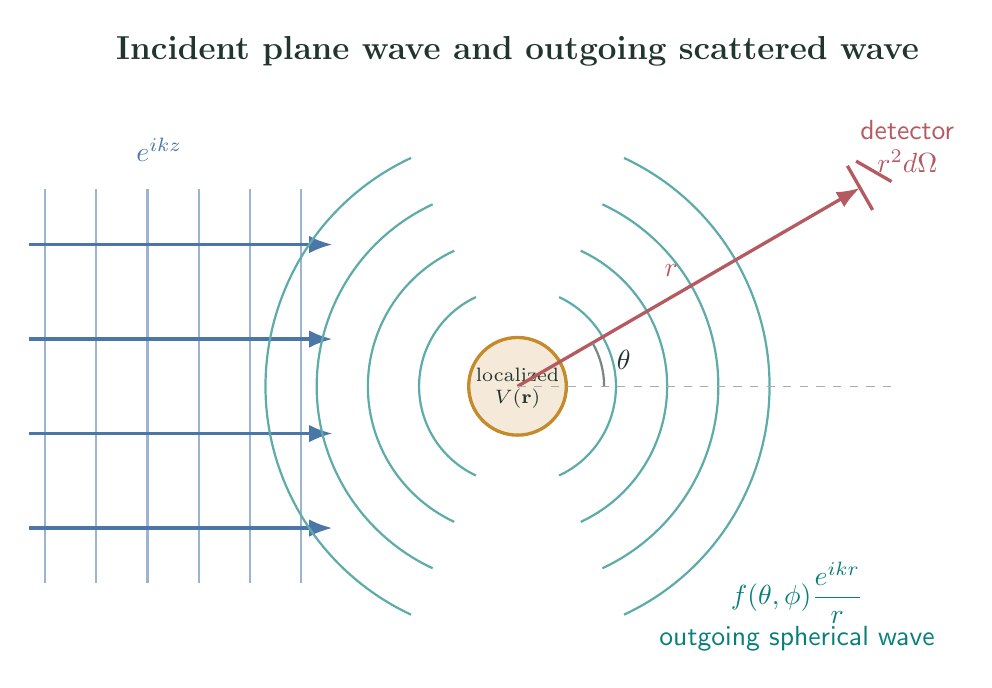
\begin{tikzpicture}[font=\sffamily,text=ink,>=Latex]
  \node[font=\bfseries\large] at (0,4.25)
    {Incident plane wave and outgoing scattered wave};
  \coordinate (O) at (0,0);

  \foreach \x in {-6.0,-5.35,-4.70,-4.05,-3.40,-2.75} {
    \draw[blue!55,thick] (\x,-2.5)--(\x,2.5);
  }
  \foreach \y in {-1.8,-.6,.6,1.8} {
    \draw[blue,very thick,->] (-6.2,\y)--(-2.35,\y);
  }
  \node[blue] at (-4.55,3.0) {$e^{ikz}$};

  \fill[gold!18] (O) circle (.62);
  \draw[gold,very thick] (O) circle (.62);
  \node[align=center,font=\scriptsize] at (0,-.02)
    {localized\\$V(\mathbf r)$};

  \foreach \r in {1.25,1.9,2.55,3.2} {
    \draw[teal!65,thick] ($(O)+(-65:\r)$)
      arc[start angle=-65,end angle=65,radius=\r];
    \draw[teal!65,thick] ($(O)+(115:\r)$)
      arc[start angle=115,end angle=245,radius=\r];
  }

  \coordinate (D) at (4.35,2.52);
  \draw[rose,very thick,->] (O)--(D)
    node[midway,above left] {$r$};
  \draw[ink!40,dashed] (O)--(4.85,0);
  \draw[ink!60,thick] (1.1,0)
    arc[start angle=0,end angle=30,radius=1.1];
  \node at (1.35,.34) {$\theta$};

  \draw[rose,very thick] ($(D)+(-.16,.28)$)--($(D)+(.16,-.28)$);
  \draw[rose,very thick] ($(D)+(-.05,.34)$)--($(D)+(.40,.08)$);
  \node[rose,align=center] at (4.95,3.05)
    {detector\\$r^2d\Omega$};
  \node[teal,align=center] at (3.55,-2.8)
    {$\displaystyle f(\theta,\phi)\frac{e^{ikr}}{r}$\\
     outgoing spherical wave};
\end{tikzpicture}
\end{document}
